\documentclass[12pt]{article}
\usepackage{hyperref}
\usepackage{listings}
\usepackage[margin=1in]{geometry}
\usepackage{enumitem}
\usepackage{multicol}
\usepackage{array}
\usepackage{titlesec}
\usepackage{helvet}
\renewcommand{\familydefault}{\sfdefault}
\usepackage{amsmath}     % For math equations
\usepackage{amssymb}     % For advanced math symbols
\usepackage{amsfonts} % For math fonts
\usepackage{gvv}
\usepackage{esint}
\usepackage[utf8]{inputenc}
\usepackage{graphicx}
\usepackage{pgfplots}
\pgfplotsset{compat=1.18}
\titleformat{\section}{\bfseries\large}{\thesection.}{1em}{}
\setlength{\parindent}{0pt}
\setlength{\parskip}{6pt}
\usepackage{multirow}
\usepackage{float}
\usepackage{caption}


\begin{document}

\textbf{Problem 4.13.101.} Let $p, q$ amd $r$ be nonzero real numbers that are the $10^{th}, 100^{th}$ and $1000^{th}$ terms of a harmonic progression, respectively. Consider the following system of linear equations

\begin{align}
x + y + z &= 1 \\
10x + 100y + 1000z &= 0 \\
qrx + pry + pqz &= 0
\end{align}

(I) If $\dfrac{q}{r} = 10$, then the system of linear equations has\\
(II) If $\dfrac{p}{r} \neq 100$, then the system of linear equations has\\
(III) If $\dfrac{p}{q} \neq 10$, then the system of linear equations has\\
(IV) If $\dfrac{p}{q} = 10$, then the system of linear equations has


(A) $x = 0,\; y = \dfrac{10}{9},\; z = -\dfrac{1}{9}$ as a solution\\
(B) $x = \dfrac{10}{9},\; y = -\dfrac{1}{9},\; z = 0$ as a solution\\
(C) infinitely many solutions\\
(D) no solution\\
(E) at least one solution


\textbf{Input Data}

\begin{table}[H]
\centering
\begin{tabular}{|l |l|}
\hline
Given scalars: & \(p,\; q,\; r\) \\
\hline
HP relation (reciprocals in AP): & \(\dfrac{1}{p}=a+9d,\; \dfrac{1}{q}=a+99d,\; \dfrac{1}{r}=a+999d\) \\
\hline
Coefficient matrix (M) rows: & $\vec R_1$=\myvec{1,1,1}, $\vec R_2$=\myvec{10,100,1000},$ \vec R_3$=\myvec{qr,pr,pq} \\
\hline
RHS vector: & $\vec{b}$=\myvec{1\\0\\0}\\
\hline
\end{tabular}
\caption{Input data (scalars and vectors) derived from problem statement}
\label{}
\end{table}


\textbf{Solution:}

Given system of equations is:

$\vec{x}$ = 
\myvec{
x \\ y \\ z
}.


% matrix equation

\myvec{
1 & 1 & 1 \\
10 & 100 & 1000 \\
qr & pr & pq
} $\vec{x}$
=
\myvec{
1 \\ 0 \\ 0
}.


\noindent\textbf{From the system of equations, the augmented matrix formed is:}

\begin{align}
[\,\myvec{M}\mid \vec b\,]
&= \myvec{1 & 1 & 1 & 1 \\
10 & 100 & 1000 & 0 \\
qr & pr & pq & 0}
\end{align}

Eliminate first-column below row1: do \(R_2\leftarrow R_2-10R_1\) and \(R_3\leftarrow R_3-(qr)R_1\):
\begin{align}
\myvec{1 & 1 & 1 & 1 \\
10 & 100 & 1000 & 0 \\
qr & pr & pq & 0}
&\xrightarrow{R_2-10R_1,\;R_3-qrR_1}
\myvec{1 & 1 & 1 & 1 \\
0 & 90 & 990 & -10 \\
0 & pr-qr & pq-qr & -qr}
\end{align}

Now eliminate the (3,2) entry using row2. Set
\begin{align}
s &= \frac{pr-qr}{90},
\end{align}
and do \(R_3\leftarrow R_3 - sR_2\). Compute the new third-row entries explicitly:

\begin{align}
(3,3)\text{: }&\quad (pq-qr) - s\cdot 990
\\
&= pq-qr - 990\cdot\frac{pr-qr}{90}
\\
&= pq-qr - 11(pr-qr)
\\
&= pq - 11\,pr + 10\,qr \;:=\; D,
\end{align}

\begin{align}
(3,4)\text{: }&\quad -qr - s(-10)
\\
&= -qr + 10\cdot\frac{pr-qr}{90}
\\
&= -qr + \frac{pr-qr}{9}
\\
&= \frac{pr - 10\,qr}{9} \;:=\; E.
\end{align}

Thus the matrix in row-echelon form is
\begin{align}
[\,\myvec{M}\mid \vec b\,] =
\myvec{1 & 1 & 1 & 1 \\
0 & 90 & 990 & -10 \\
0 & 0 & D & E},
\end{align}
with
\begin{align}
D &= pq - 11\,pr + 10\,qr, \qquad E = \frac{pr - 10\,qr}{9}.
\end{align}

Conclusions from the echelon form (standard linear algebra facts):
\begin{align}
&\text{If } D\neq 0,\ \text{the system has a unique solution.} \notag \\
&\text{If } D=0 \text{ but } E\neq 0,\ \text{the system is inconsistent (no solution).} \notag \\
&\text{If } D=0 \text{ and } E=0,\ \text{the system has infinitely many solutions (rank 2).} \notag
\end{align}


\noindent\textbf{Using the HP condition,}

Because \(p,q,r\) are the \(10^{\text{th}},100^{\text{th}},1000^{\text{th}}\) terms of an HP,
\begin{align}
\frac{1}{p}=a+9d,\qquad \frac{1}{q}=a+99d,\qquad \frac{1}{r}=a+999d
\end{align}
for some real \(a,d\). Evaluate \(D/(pqr)\) to simplify algebra:
\begin{align}
\frac{D}{pqr}
&= \frac{1}{r} - \frac{11}{q} + \frac{10}{p}
\\
&= (a+999d) - 11(a+99d) + 10(a+9d)
\\
&= a + 999d -11a -1089d +10a +90d = 0.
\end{align}
Hence
\begin{align}
\boxed{D\equiv 0\ \text{for every valid HP triple }(p,q,r).}
\end{align}
Therefore the coefficient matrix is singular and a unique solution is impossible.

Next compute \(E/(pqr)\):
\begin{align}
\frac{E}{pqr}
&= \frac{1}{9}\Big(\frac{1}{q} - \frac{10}{p}\Big)
\\
&= \frac{1}{9}\big( (a+99d) - 10(a+9d)\big)
\\
&= \frac{1}{9}(-9a + 9d) = d-a.
\end{align}
Thus
\begin{align}
\boxed{E = pqr\,(d-a).}
\end{align}
So the system is consistent (infinitely many solutions) exactly when \(E=0\), i.e. when \(d=a\). Equivalently,
\begin{align}
d=a \quad\Longrightarrow\quad \frac{1}{p}=10a,\ \frac{1}{q}=100a,\ \frac{1}{r}=1000a
\quad\Longrightarrow\quad p:q:r = 100:10:1.
\end{align}

\noindent\textbf{Parametric solution when consistent.} If \(d=a\) (equivalently \(p:q:r=100:10:1\)) then the third equation is redundant and we can solve the first two:
\begin{align}
x+y+z &= 1, \\
10x+100y+1000z &= 0.
\end{align}
Set \(z=t\). Then \(y=1-t-x\). Substitute into the second:
\begin{align}
10x + 100(1-t-x) &= -1000t
\\
-90x +100 -100t &= -1000t
\\
-90x &= -900t -100
\\
x &= 10t + \frac{10}{9}.
\end{align}
Thus the solution family is
\begin{align}
\vec{x} = \myvec{10t+\frac{10}{9}\\ -11t-\frac{1}{9}\\ t},\qquad t\in\mathbb{R}.
\end{align}
Two convenient particular choices:
\begin{align}
t=-\frac{1}{9} &\implies \vec{x}=\myvec{0\\\frac{10}{9}\\ -\frac{1}{9}}\quad\text{(matches option A)},\\
t=0 &\implies \vec{x}=\myvec{\frac{10}{9}\\ -\frac{1}{9}\\ 0}\quad\text{(matches option B)}.
\end{align}

So when consistent both A and B are valid particular solutions, and there are infinitely many of them (C).


\noindent\textbf{Now check cases (I)--(IV) }


\noindent\textbf{(I) If } $\dfrac{q}{r}=10$.

From reciprocals,
\begin{align}
\frac{1/q}{1/r} = \frac{r}{q} = \frac{1}{10} \quad\Longrightarrow\quad
\frac{a+99d}{a+999d} = \frac{1}{10}.
\end{align}
Multiply out:
\begin{align}
10(a+99d) = a+999d \quad\Longrightarrow\quad 10a+990d = a+999d \quad\Longrightarrow\quad 9a = 9d,
\end{align}
so \(a=d\). Therefore \(E=0\) and we are in the consistent case. Conclusion:
\begin{align}
\text{(I)}\quad\boxed{\text{infinitely many solutions (option C). \ Also A and B are solutions.}}
\end{align}


\noindent\textbf{(II) If } $\dfrac{p}{r}\neq 100$.

Now \(p/r\neq100\) means \(p\neq100r\). Under the HP parametrisation, \(p=100r\) is equivalent to \(a=d\) (see derivation above). Hence \(p\neq100r\) is equivalent to \(a\neq d\). Then \(E = pqr(d-a)\neq0\). Since we already have \(D\equiv0\), \(D=0\) and \(E\neq0\) implies inconsistency. Conclusion:
\begin{align}
\text{(II)}\quad\boxed{\text{no solution (option D).}}
\end{align}



\noindent\textbf{(III) If } $\dfrac{p}{q}\neq 10$.

Similarly \(p/q = 10\) is equivalent to \(a=d\) (check by \((a+9d)/(a+99d)=1/10\) as in (I)). Therefore \(p/q\neq10\) implies \(a\neq d\) and hence \(E\neq0\). With \(D\equiv0\) this gives inconsistency. Conclusion:
\begin{align}
\text{(III)}\quad\boxed{\text{no solution (option D).}}
\end{align}


\noindent\textbf{(IV) If } $\dfrac{p}{q}=10$.

As noted, \(p/q=10\) implies \(a=d\). Thus \(E=0\) and the system is consistent with infinitely many solutions. Conclusion:
\begin{align}
\text{(IV)}\quad\boxed{\text{infinitely many solutions (option C). \ Also A and B are solutions.}}
\end{align}

\begin{figure}[H]
    \centering
    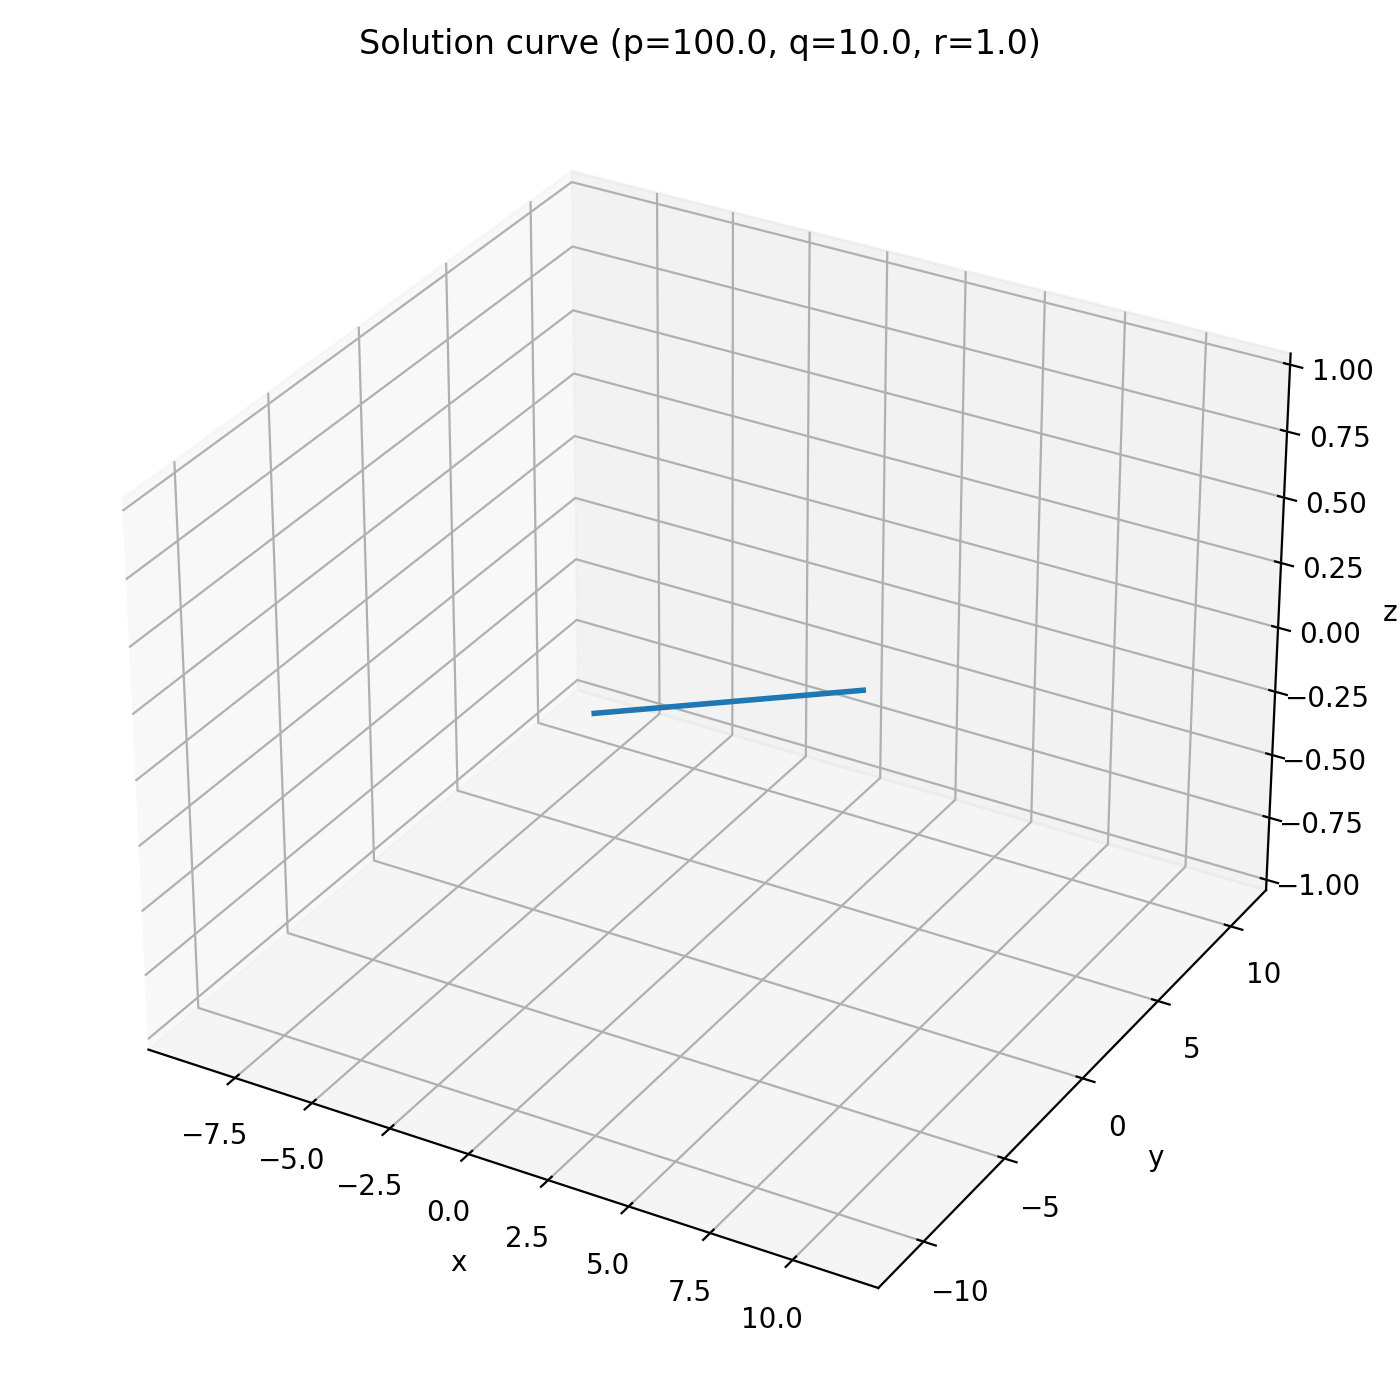
\includegraphics[width=0.9\columnwidth]{figs/hp_3d_only.png}
    \caption{}
    \label{fig:placeholder}
\end{figure}



\end{document}
